\section{Methods}  
    In this section, a concise overview is given of the three simulation methods—MC simulation, manual-IS, and MCMC-IS. These methods are employed for the generation of a representative hazard scenario, and their respective mathematical explanations are explored. 

    \subsection{Overview of Simulation Methods}
        MC simulations are fundamental in probabilistic modeling. These simulations employ random sampling from specified probability distributions to estimate outcomes and quantify uncertainties in complex systems. In the context of community resilience and natural hazards, the term "probability distribution" represents the likelihood of different hazard intensities, while "estimate" refers to the expected loss to the community due to the natural hazard. These simulations are particularly valuable in assessing the impact of potential hazards on communities and in planning for resilience.

        However, a challenge arises when sampling rare but highly consequential events, such as severe natural hazards. In these cases, the variance in the MC estimates can be quite high, leading to less confidence in the simulation results. 

        To address this issue and reduce the variance of the estimates, two main strategies are available. The first strategy involves increasing the number of simulations. This approach is grounded in the Law of Large Numbers, which suggests that a larger sample size can lead to more accurate estimates. However, this method can be computationally expensive or impractical. The second strategy is to sample from an alternative distribution, a technique central to IS. IS involves drawing samples from a biased distribution that over-represents the rare, significant events, known as the \textit{importance distribution}. By assigning more weight to outcomes with a greater impact on the estimate, IS can potentially reduce variance without the need for an increased number of simulations.

        The success of IS hinges on the choice of the importance distribution. In theory, there exists an "optimal" importance distribution that would yield an estimator with zero variance. This optimal distribution, often referred to as the zero-variance distribution, would align perfectly with the function being estimated, scaled by the target distribution. Such a distribution would sample the input space in a way that each sample contributes uniformly to the estimate, eliminating the estimator's variance entirely.
        
        While the zero-variance distribution is a theoretical ideal and not attainable in practice, it serves as a guiding principle in the search for a practical importance distribution that minimizes variance as much as possible. By approximating this optimal importance distribution, we can significantly improve the efficiency and reliability of our simulations.

        The choice of the importance distribution depends on both the type of loss function and the original probability distribution, which represents the likelihood of different hazard intensities. To elucidate this concept and explore suitable importance distributions for various loss functions, we examine scenarios that depict different types of loss functions commonly encountered in the context of natural hazards. In each scenario, the loss function and original distribution are intentionally chosen to be simple, enabling the analytical determination of the optimal importance distribution. These optimal distributions are then displayed alongside the original distribution to highlight the distinctions between them.

            \begin{figure}[H]
        \centering
        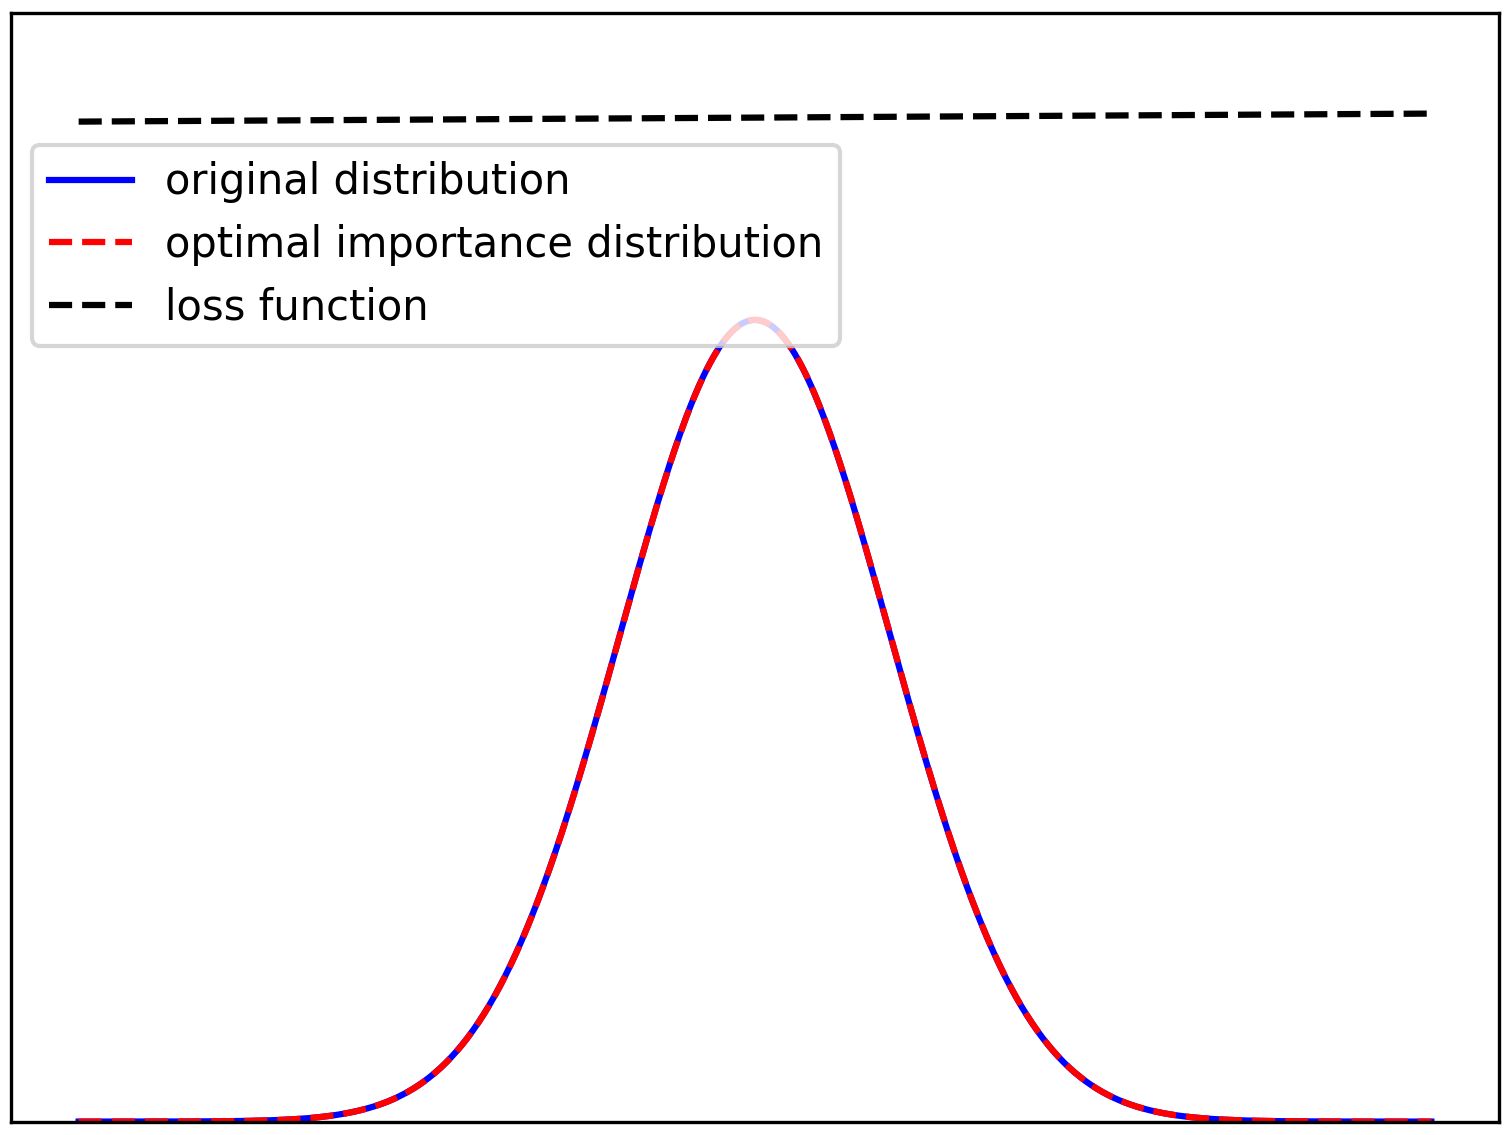
\includegraphics[scale=0.50]{Manuscript/Figures/Images/Methods/optimal_IS_dist_case1.png}
        \caption{Optimal importance distribution for a scenario with constant loss across all hazard intensities}
        \label{fig:optimal_IS_dist_case1}
    \end{figure}
        
        In Figure~\ref{fig:optimal_IS_dist_case1}, we illustrate the case where the loss is constant for all hazard intensities, such as in a floodplain where all properties are equally protected by a high-standard levee system. In this scenario, the optimal importance distribution is the same as the original distribution, indicating that MC simulation is sufficient and there is no need for IS.

            \begin{figure}[H]
        \centering
        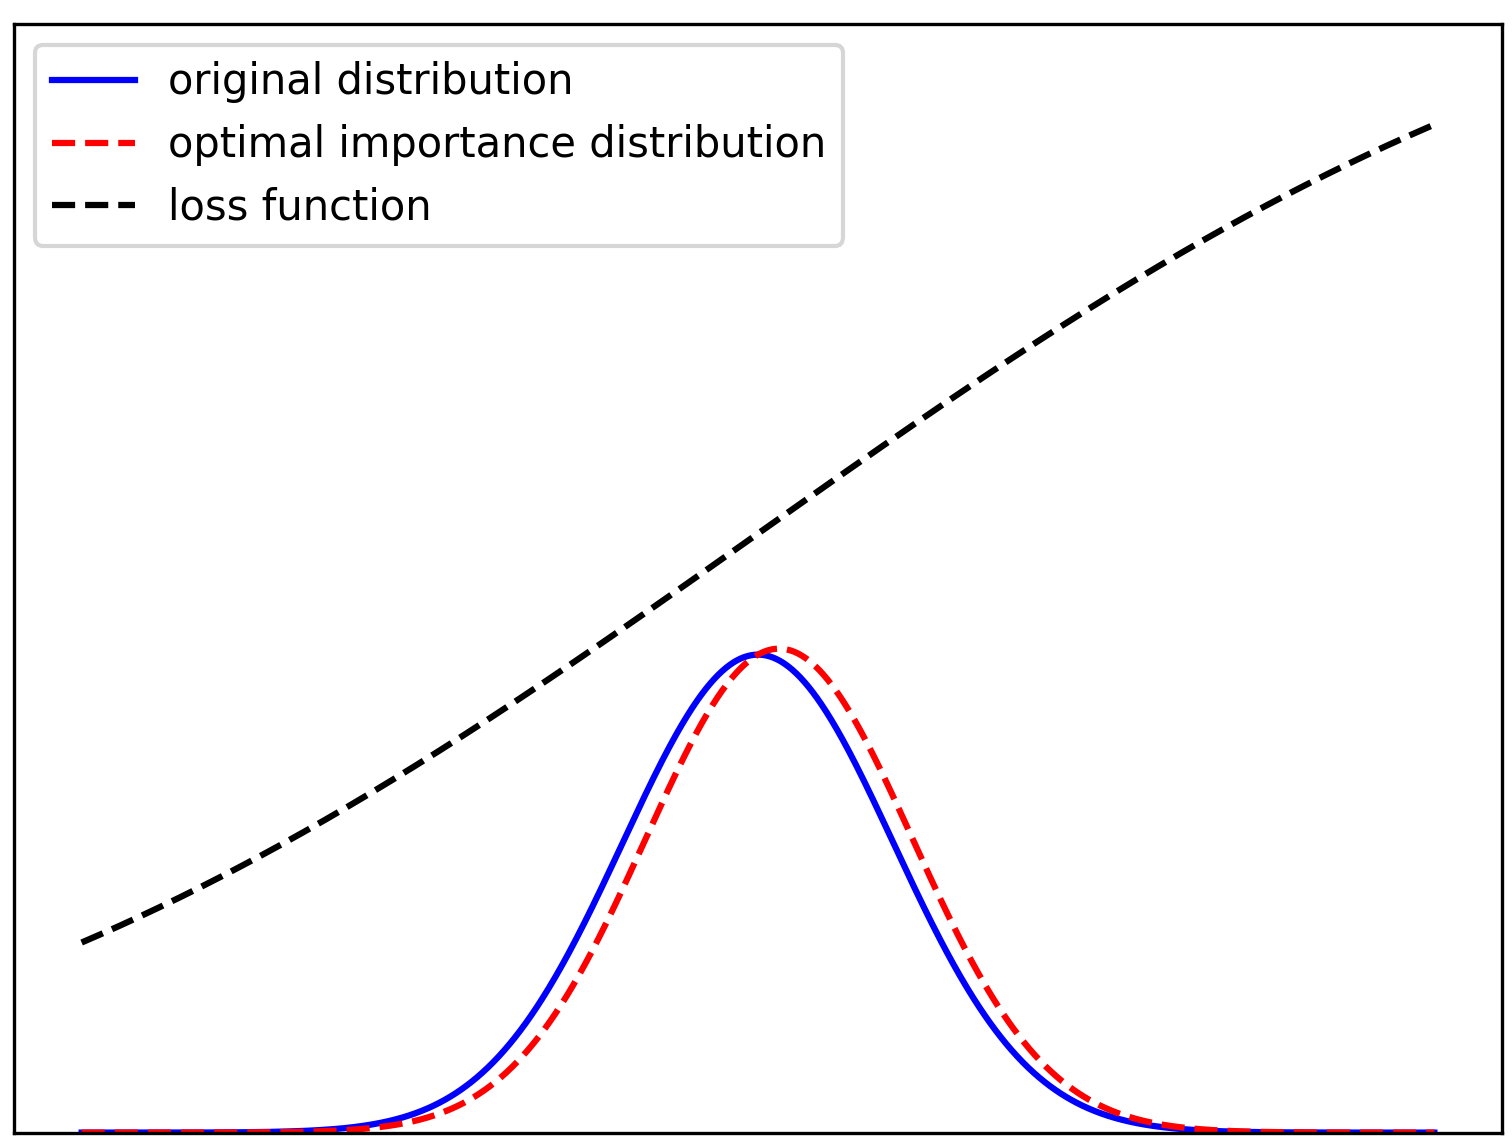
\includegraphics[scale=0.50]{Manuscript/Figures/Images/Methods/optimal_IS_dist_case2.png}
        \caption{Optimal importance distribution for a scenario with a linear loss function}
        \label{fig:optimal_IS_dist_case2}
    \end{figure}
        
        Figure~\ref{fig:optimal_IS_dist_case2} demonstrates a scenario where the loss function is almost linear over the range of the original distribution, with a slight shift to the right. This could represent a situation where the damage from a hazard increases linearly with its intensity, like the cost of repairs for minor wind damage to a building. The optimal importance distribution in this case is the same family as the original distribution but is shifted slightly to the right.

            \begin{figure}[H]
        \centering
        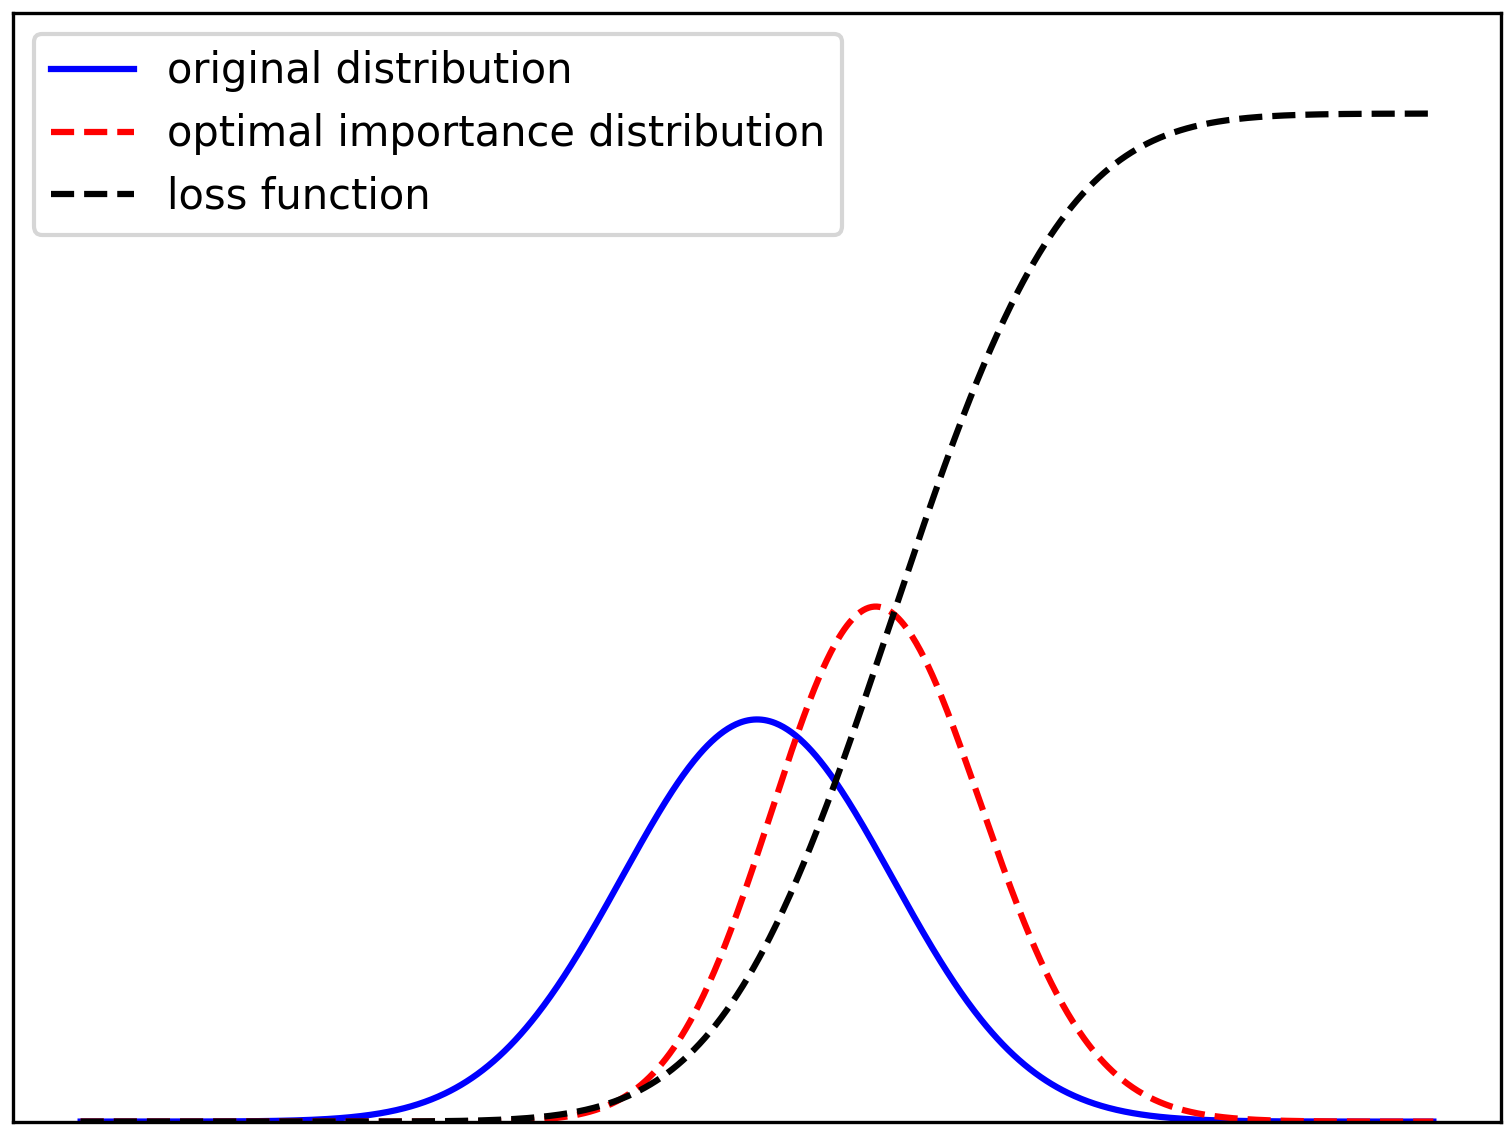
\includegraphics[scale=0.50]{Manuscript/Figures/Images/Methods/optimal_IS_dist_case3.png}
        \caption{Optimal importance distribution for a scenario with a normally distributed loss function}
        \label{fig:optimal_IS_dist_case3}
    \end{figure}
        
        In Figure~\ref{fig:optimal_IS_dist_case3}, we present a classic case where the loss function is well-represented by a normal distribution, such as the economic impact of a moderate earthquake on a region. The optimal importance distribution is shifted to the right and is tighter compared to the original distribution, suggesting that both shifting and narrowing the distribution are necessary for efficient sampling.

            \begin{figure}[H]
        \centering
        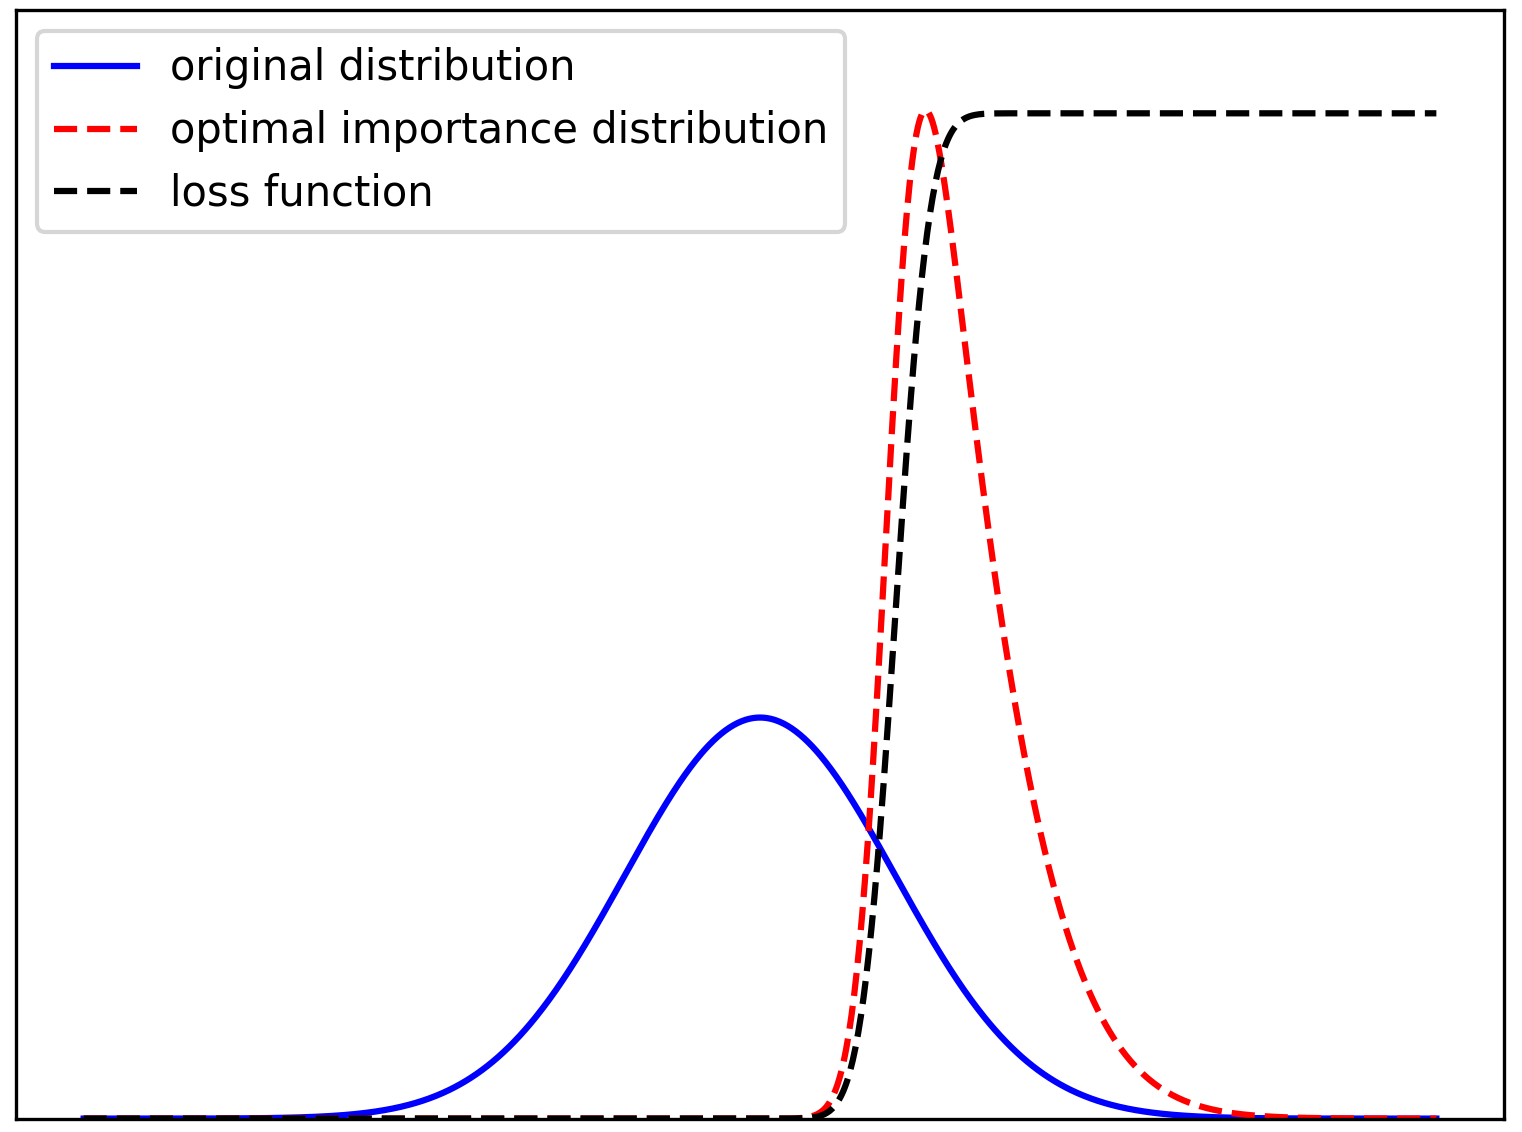
\includegraphics[scale=0.50]{Manuscript/Figures/Images/Methods/optimal_IS_dist_case4.png}
        \caption{Optimal importance distribution for a scenario with a skewed loss function}
        \label{fig:optimal_IS_dist_case4}
    \end{figure}

        Figure~\ref{fig:optimal_IS_dist_case4} depicts a scenario with a clearly skewed loss function, which might occur in the impact of a severe storm on a coastal area. The optimal importance distribution must account for this skewness to efficiently sample the important regions.

            \begin{figure}[H]
        \centering
        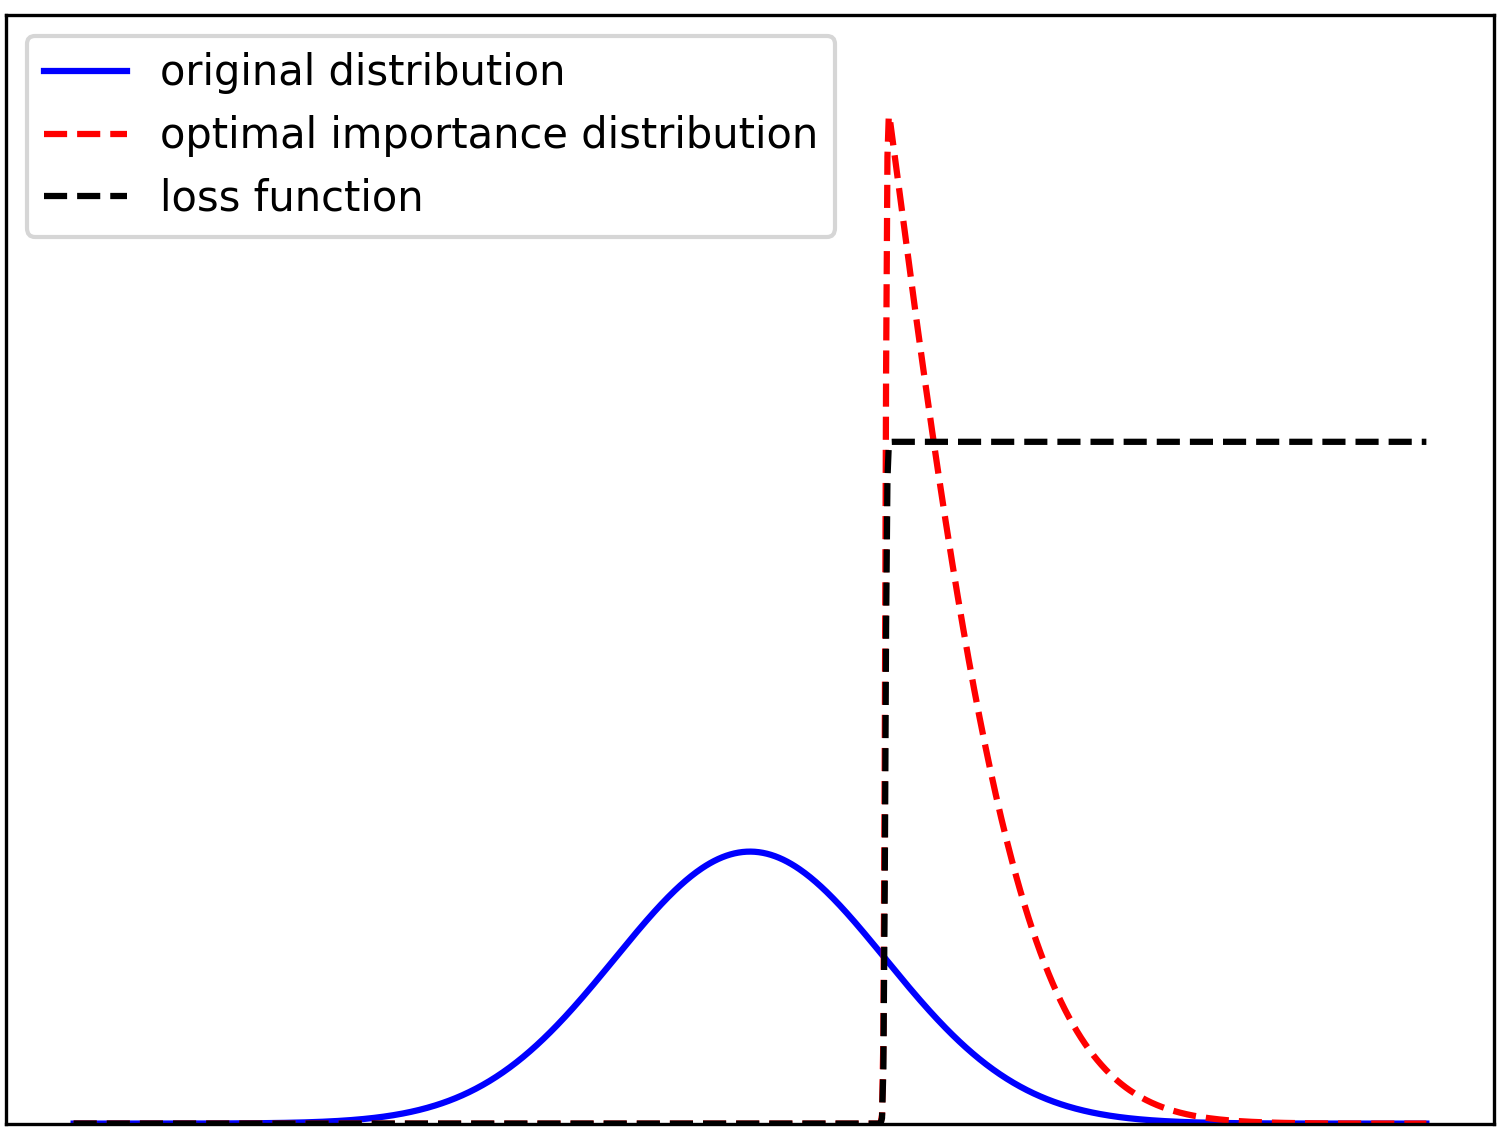
\includegraphics[scale=0.50]{Manuscript/Figures/Images/Methods/optimal_IS_dist_case5.png}
        \caption{Optimal importance distribution for a scenario with an extremely tight loss function}
        \label{fig:optimal_IS_dist_case5}
    \end{figure}
        
        Lastly, Figure~\ref{fig:optimal_IS_dist_case5} shows a situation where the loss function is extremely tight, leading to a tail-heavy distribution. This could represent the catastrophic failure of a critical infrastructure component under extreme stress. In this case, the optimal importance distribution is focused on the tail of the original distribution, indicating that tail MC might be optimal if the tail region can be identified.
        
        Having explored the influence of different loss functions on the choice of the optimal importance distribution, we now turn our attention to the methods available for approximating these distributions. Several techniques exist for this purpose, some of which involve a manual trial-and-error process. In this paper, this method is referred to as manual-IS. In the manual-IS, importance distribution can be selected from the same family distribution as the original distribution but with different parameters. Notable examples include mean translation (MT), variance scaling (VS), and a combination of both approaches \cite{lu_improved_1988}, which are visually represented in Figure~\ref{fig:IS_techniques}.    
            \begin{figure}[H]
        \centering
        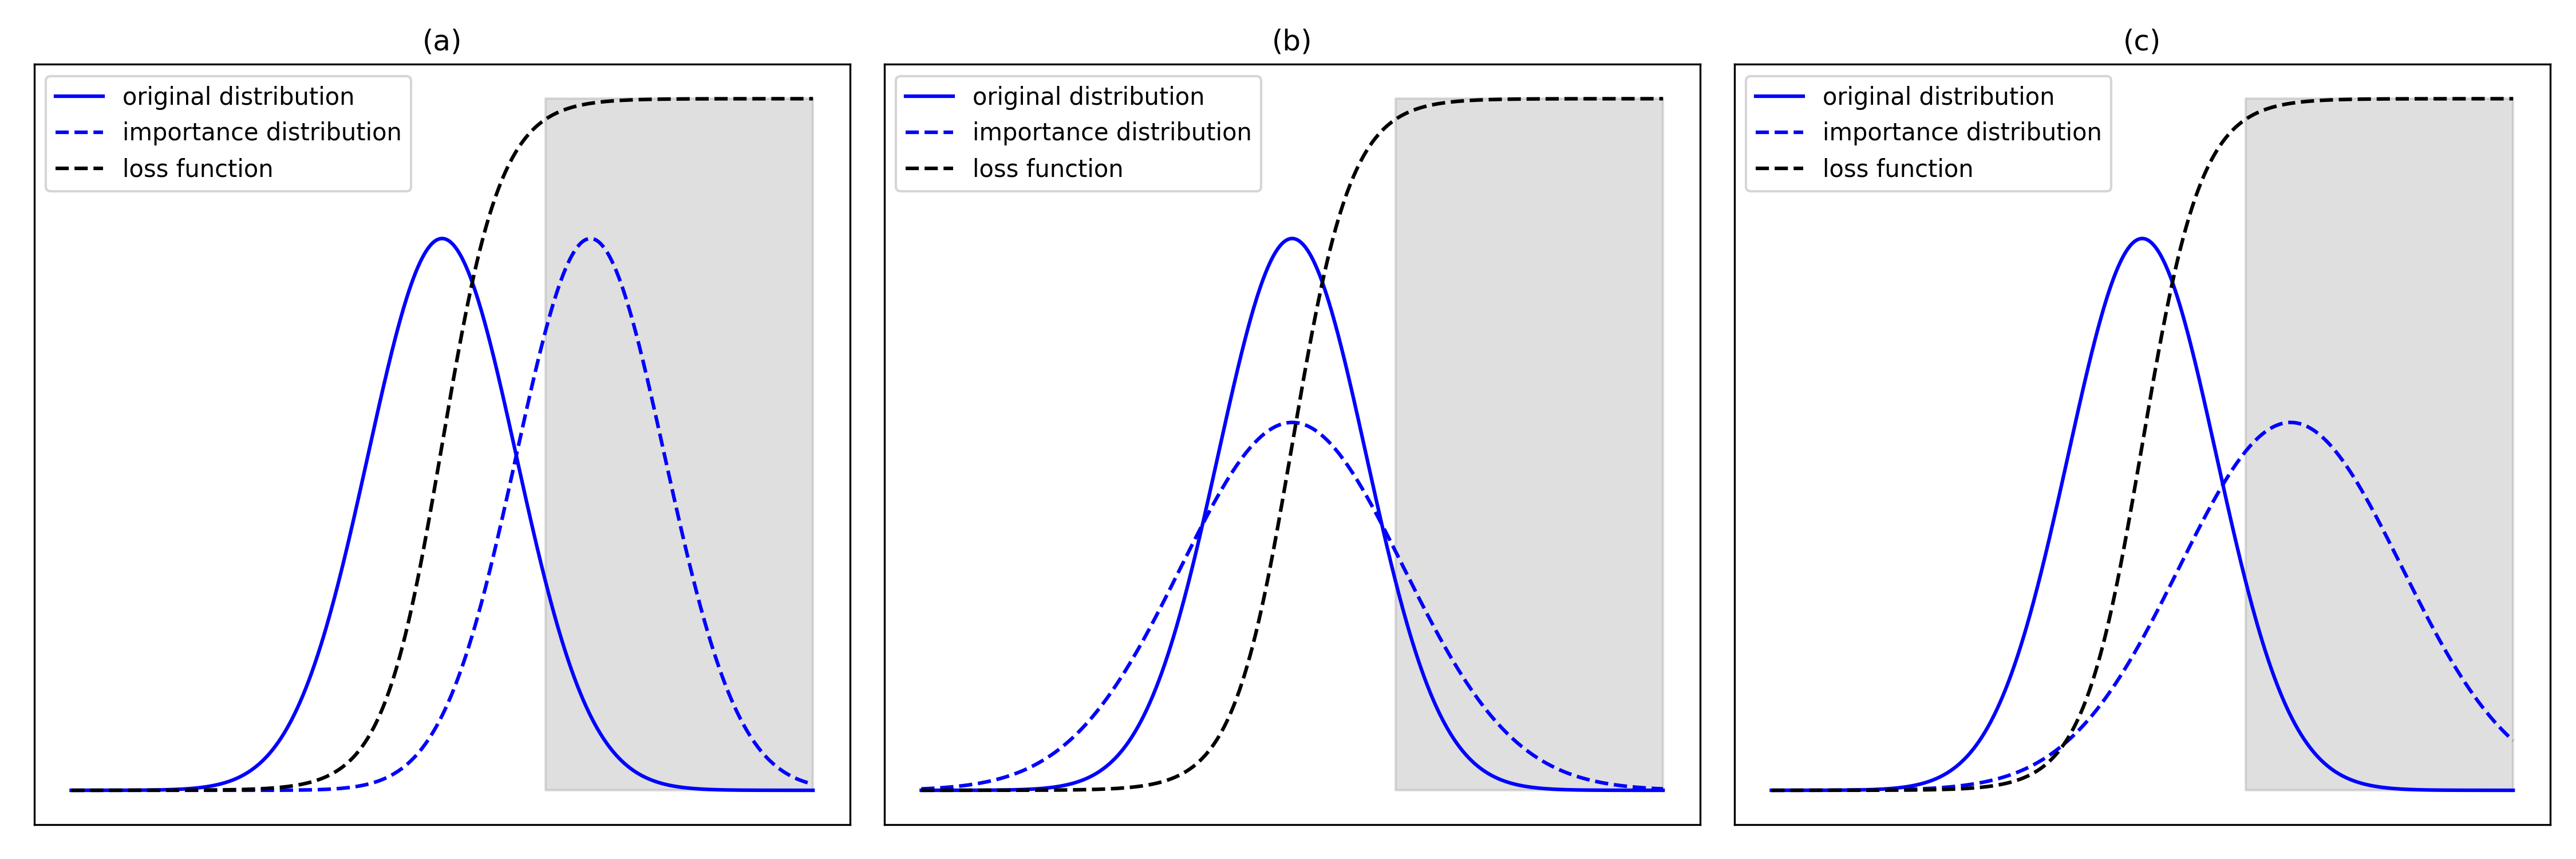
\includegraphics[scale=0.40]{Figures/Images/Methods/IS_techniques.png}
        \caption{Schematic diagrams illustrating (a) mean translation (MT), (b) variance scaling (VS), and (c) their combined application in one dimension. The shaded area denotes the effective probability density employed in importance sampling \protect\cite{lu_improved_1988}}
        \label{fig:IS_techniques}
    \end{figure}
        
        As illustrated in Figure~\ref{fig:IS_techniques}, samples associated with high values of the loss function are situated in the tail region of the original distribution, where the probability of occurrence is significantly low. In such scenarios, generating more important samples with greater frequency is advantageous. This rationale underlies the mean translation technique, where the importance distribution is aligned with the same probability distribution function as the original distribution but with a shifted mean towards the more consequential area.
        
        Alternatively, another approach to increase sampling frequency is to expand the variance of the original distribution to generate more samples in the tail region. This concept is central to the variance scaling technique. Furthermore, the combination of mean translation and variance scaling can optimize importance sampling efficiency by adjusting both the mean and variance of the importance distribution.
        
        However, the manual trial-and-error process for estimating the importance density function can be time-consuming, often requiring multiple iterations to approximate the optimal importance distribution. To address this challenge, alternative methods have been proposed for systematically estimating near-optimal importance distributions. One such method is known as MCMC-IS, introduced by Parpas et al. \cite{parpas_importance_2015}, which combines Markov Chain Monte Carlo techniques with importance sampling to iteratively refine the importance distribution.

        The MCMC-IS framework comprises three essential steps:
        \begin{enumerate}
            \item Generation of samples from a distribution that aims to minimize variance, referred to as a "zero-variance distribution", using a Markov Chain Monte Carlo (MCMC) algorithm.
            \item Construction of an approximate zero-variance distribution through Kernel Density Estimation (KDE) algorithm.
            \item Sampling from the approximate zero-variance distribution to produce a lower-variance importance sampling estimate.
        \end{enumerate}

        The first crucial step in the MCMC-IS framework involves the generation of samples using the MCMC method. MCMC is a powerful adaptive sampling technique widely used for approximating complex probability distributions. It operates by iteratively updating the current state based on a proposal distribution, thereby exploring the target distribution of interest. There exist several MCMC algorithms, each tailored to specific scenarios and distributions \cite{gelman_handbook_2010}. In this study, we employ the Metropolis-Hastings algorithm for MCMC sampling. The Metropolis-Hastings algorithm is a widely used choice due to its simplicity of implementation and flexibility \cite{parpas_importance_2015}. It involves generating new samples from a proposal distribution and accepting or rejecting them based on a ratio of the proposed sample's probability to that of the previous sample to ensure the generated samples eventually resemble the target distribution.
        
        However, a significant challenge is picking the right parameters for proposal distribution, like proposal variances, to make the mixing and convergence efficient. To address this challenge, the adaptive Metropolis-Hastings algorithm has emerged as a promising solution, particularly within the MCMC-IS framework. This adaptive technique offers a dynamic approach to adjusting the parameters of MCMC algorithms as they run, effectively enabling the algorithms to "learn" and adapt to better parameter values for more efficient sampling \cite{haario_adaptive_2001}. In this approach, the covariance matrix within the proposal distribution is updated after each chunk of iterations to better reflect the correlations between random variables. The proposal distribution at iteration $n$ is as follows, but for a more detailed explanation, refer to \cite{haario_adaptive_2001}:
        $$Q_n(x, \mu)=\mathcal{N}(\mu,{(0.1)}^2I_d/d)\quad \text{for} \quad n\le2d$$
        $$Q_n(x, \mu)=(1-\beta)\mathcal{N}(\mu,{(2.38)}^2\Sigma_n/d) + \beta\mathcal{N}(\mu,{(0.1)}^2I_d/d)\quad \text{for} \quad n>2d$$
        where,
        $Q_n(x, \mu)$ is the proposal distribution at iteration $n$, which generates candidate samples $x$ based on the current state $\mu$;
        $\mathcal{N}(\mu, \sigma^2)$ is the Gaussian distribution with mean $\mu$ and variance $\sigma^2$, used as a building block for constructing the proposal distribution;\\
        $0.1$ is a fixed constant used to set the variance for the proposal distribution when $n$ is less than or equal to $2d$;
        $I_d$ is the identity matrix of dimension $d$;       
        $\beta$ is a weighting factor that blends two Gaussian distributions within the proposal distribution when $n$ is greater than $2d$;      
        $2.38$ is a scaling factor used to adjust the variance of the Gaussian component of the proposal distribution when $n$ is greater than $2d$;        
        $\Sigma_n$ is the covariance matrix updated after each chunk of iterations to better reflect the correlations between random variables.        
        
        Following the generation of MCMC samples, the subsequent step is to construct an approximate zero-variance distribution using the KDE algorithm. KDE is a statistical technique used to estimate the probability density function of a random variable based on the provided samples. KDE relies on two primary parameters: the choice of a kernel function and the bandwidth parameter. The kernel function determines the shape of the kernels placed on each data point, while the bandwidth parameter controls the width of these kernels. The selection of appropriate kernel functions and bandwidth values is essential, as it directly impacts the quality of the estimated importance density.
   
    \subsection{Mathematical Expressions}
        Let $x$ represent a random variable (or vector) characterized by a (joint) probability density function $p(x)$. The primary objective is to obtain the moments, specifically the mean and variance, of the function $h = f(x)$, where $f$ stands for a specified deterministic function (operator). The mean ($\mu_h$) and variance ($\sigma_h^2$) of $h$ can be expressed as follows:
        $$\mu_h=E[h]=E[f(x)]=\int_\Omega f(x)p(x)dx$$
        $$\sigma_h^2=E{[f(x)-\mu_h]^2}=\int_\Omega[f(x)-\mu_h]^2 p(x)dx = \int_\Omega f^2(x)p(x)dx-\mu^2_h$$
        Where, $\Omega$ is a probability space, $E$ represents statistical expectation.
        
        For the estimation of $\mu_h$ using the MC method, a set of samples $(x_i,\quad i=1,2,…,N)$ is randomly drawn from the density function $p(x)$, and the function mean $(\mu_{MC})$ and variance $(\sigma_{MC}^2)$ are computed as follows:
        $$\mu_{MC}=\frac{1}{N}\sum_{i=1}^{N} f(x_i)$$
        $$\sigma_{MC}^2=\frac{1}{N}\sum_{i=1}^{N}f^2(x_i)-(\frac{1}{N}\sum_{i=1}^{N} f(x_i))^2$$
        Where $\mu_{MC}$ and $\sigma_{MC}^2$ are the mean and variance of $h=f(x)$ estimated using the MC simulation method, respectively.
        
        Sometimes, achieving accurate estimations can be challenging for two primary reasons. First, the original distribution may be difficult to sample from, posing inherent computational complexities. Second, accuracy may be compromised when the function $f(x)$ exhibits high values in regions where the probability density function $p(x)$ is low. This latter scenario is particularly prevalent when dealing with natural hazards, where extreme events occur with low probability. In these situations, importance sampling becomes advantageous due to its potential to find accurate estimations more rapidly compared to MC methods. Suppose we draw samples, $(x_i, \quad i=1,2,…,N)$, from an importance density function $q(x)$ rather than the original density function $p(x)$, with $q(x)$ being zero only where $p(x)$ is zero. To correct for the bias and maintain the mean, the original function $f(x)$ is adjusted by introducing a modified function, denoted as $f_q(x)$:
        $$f_q(x)=f(x) w(x)$$
        Where $w(x)=p(x)/q(x)$ is called a weight function. 
        The mean and variance of f(x) can also be written as:
        $$\mu_{IS}=\frac{1}{N} \sum_{i=1}^{N}f(x_i)w(x_i)$$
        $$\sigma_{IS}^2=\frac{1}{N} \sum_{i=1}^N f^2(x_i)w^2(x_i)-\mu_{IS}^2$$
        Where $\mu_{IS}$ and $\sigma_{IS}^2$ are the mean and variance of $h=f(x)$ estimated using the IS simulation method, respectively. 
        
        

        % MC simulations, a cornerstone of probabilistic modeling, rely on random sampling from specified probability distributions to estimate outcomes and assess uncertainties. The MC method provides a robust framework for exploring a broad range of scenarios, making it particularly valuable when dealing with intricate systems characterized by multiple sources of variability. On the other hand, IS represents a specialized adaptation of the MC method. The fundamental concept behind importance sampling lies in recognizing that certain random input variables or vectors exert a more significant influence on the estimated quantity than others. To mitigate the estimator's variance, it is advantageous to sample these "important" values more frequently, which can be achieved by drawing samples from a biased density function. Subsequently, the simulation results are appropriately weighted to counteract the bias introduced by sampling from this skewed density function.
    
        % Importance sampling techniques involve two primary steps. The first step entails a modification of the initial sampling procedure. To allocate more samples to "important" regions within the sample space, samples are generated from an alternative probability density function referred to as an \textit{importance density function}. The second step focuses on rectifying the introduced bias by averaging the outcomes of various samples (realizations) while applying weights associated with the bias. This process ensures that the estimated quantity maintains its true mean, thereby eliminating distortion caused by the biased sampling approach.

        % While IS can often lead to estimates with significantly lower variance compared to their MC counterparts, it's important to note that this reduction in variance is not guaranteed. The effectiveness of IS relies heavily on the selection of an appropriate importance density function, which remains a challenging and non-generalizable process. This issue has been a central focus of numerous papers in the fields of statistics and simulation.
    
        % The choice of the importance density function should be made with the dual objectives of minimizing the estimated variance quantity and reducing the computational effort required to estimate the mean quantity. However, directly minimizing the variance of importance sampling estimation as a function of the unknown density function is a complex task.











